\begin{figure}[p]
	\centering

	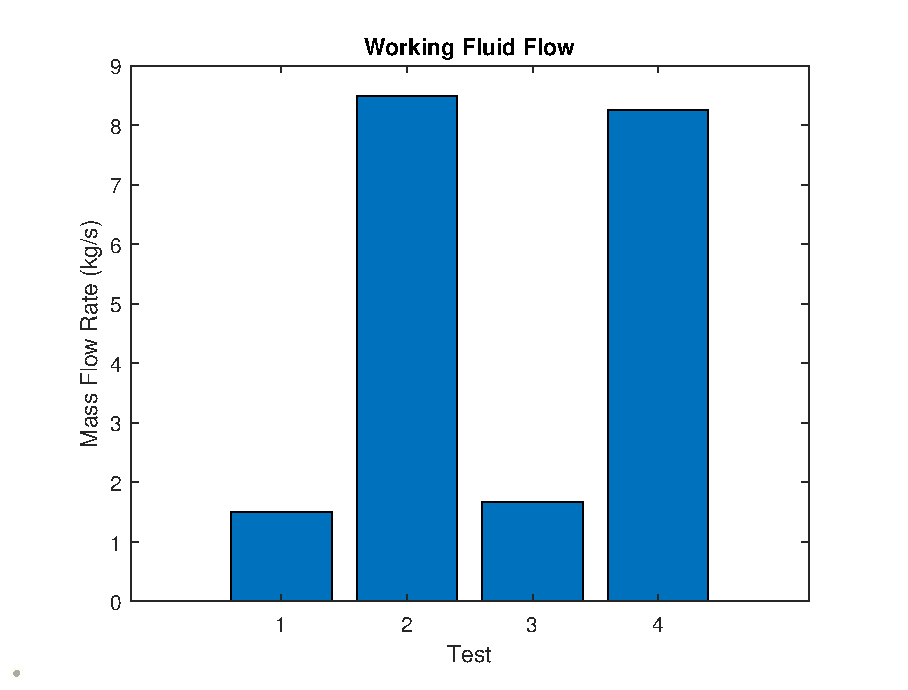
\includegraphics[width=\textwidth]{figures/gfFlow}

	\caption{Comparison of working fluid mass flow rates for the greenfield case of the ORC prime power system model. All test assume a source temperatures of \SI{364.5}{\kelvin} (\SI{91}{\degreeCelsius}), and source and sink flow rates of \SI{940}{\liter\per\minute}. Tests 1 and 2 use a heat sink temperature of \SI{281.6}{\kelvin} (\SI{8.5}{\degreeCelsius}), while tests 3 and 4 use \SI{276.6}{\kelvin} (\SI{3.5}{\degreeCelsius}). The power setpoints of the four tests are \SIlist{27.5;40.0;30.8;42.0}{\kilo\watt}. Tests 1 and 3 use the maximum power setpoint while also ensuring the working fluid fully evaporates in the evaporator. Tests 2 and 4 use the maximum power setpoint while maintaining a stable simulation. }
	%Psetpoint[2.75e4;4.0e4;3.08e4;4.2e4;]
	\label{fig:gfFlow}
\end{figure}